\documentclass{beamer}

\usepackage[utf8]{inputenc}
\usepackage[T1]{fontenc}
\usepackage{mathtools,tikz,tikzscale}
\usepackage{wrapfig}
\usepackage[labelformat=simple]{subcaption}
% \usepackage[hidelinks]{hyperref}

\usetheme{Madrid}
% \useoutertheme{infolines}
\beamertemplatenavigationsymbolsempty


\title{Quantum Snowflake}
\subtitle{Bachelor's Thesis Presentation}
\author{Viktor Qvarfordt}
\institute[]{Department of Mathematics, Department of Physics\\Stockholm University}
\date{May 19, 2015}
\subject{Mathematical Physics}


% \setbeamertemplate{headline}
% {
%   \leavevmode%
%   \hbox{%
%   \begin{beamercolorbox}[wd=.5\paperwidth,ht=2.25ex,dp=1ex,center]{section in head/foot}%
%     \usebeamerfont{subsection in head/foot}\hspace*{2ex}\insertshorttitle
%   \end{beamercolorbox}%
%   \begin{beamercolorbox}[wd=.5\paperwidth,ht=2.25ex,dp=1ex,center]{subsection in head/foot}%
%     \usebeamerfont{section in head/foot}\insertsectionhead\ifx\insertsubsectionhead\empty\else~/~\insertsubsectionhead\fi\hspace*{2ex}
%   \end{beamercolorbox}}%
%   \vskip0pt%
% }

\makeatletter
\setbeamertemplate{footline}
{
  \leavevmode%
  \hbox{%
  \begin{beamercolorbox}[wd=.3\paperwidth,ht=2.25ex,dp=1ex,center]{author in head/foot}%
    \usebeamerfont{author in head/foot}\insertshortauthor
  \end{beamercolorbox}%
  \begin{beamercolorbox}[wd=.4\paperwidth,ht=2.25ex,dp=1ex,center]{title in head/foot}%
    \ifx\insertsectionhead\empty\inserttitle\else%
    \insertsectionhead\ifx\insertsubsectionhead\empty\else~/~\insertsubsectionhead\fi%
    \fi
  \end{beamercolorbox}%
  \begin{beamercolorbox}[wd=.3\paperwidth,ht=2.25ex,dp=1ex,center]{date in head/foot}%
    \usebeamerfont{date in head/foot}\insertshortdate{}\hspace*{2em}\raggedleft
    \insertframenumber{} / \inserttotalframenumber\hspace*{2ex}
  \end{beamercolorbox}}%
  \vskip0pt%
}
\makeatother

\makeatletter\let\frametextheight\beamer@frametextheight\makeatother

\newcommand{\Dom}{\operatorname{Dom}}
\newcommand{\Ran}{\operatorname{Ran}}
\newcommand{\Ker}{\operatorname{Ker}}
\newcommand{\Tr}{\operatorname{Tr}}
\newcommand{\norm}[1]{\left\lVert#1\right\rVert}
\newcommand{\Norm}[1]{\lVert#1\rVert}
\newcommand{\abs}[1]{\left\lvert#1\right\rvert}
\newcommand{\ip}[2]{\ensuremath{\langle #1, #2 \rangle}}

\newcommand{\Z}{\mathbb{Z}}
\newcommand{\R}{\mathbb{R}}
\newcommand{\C}{\mathbb{C}}
\renewcommand{\H}{\mathcal{H}}

\newcommand{\D}[2]{\frac{d#1}{d#2}}
\newcommand{\pD}[2]{\frac{\partial#1}{\partial#2}}

\newcommand{\Dn}[3]{\frac{d^#3#1}{d#2^#3}}
\newcommand{\pDn}[3]{\frac{\partial^#3#1}{\partial#2^#3}}

\newcommand{\Dop}[1]{\frac{d}{d#1}}
\newcommand{\pDop}[1]{\frac{\partial}{\partial#1}}

\newcommand{\Dopn}[2]{\frac{d^#2}{d#1^#2}}
\newcommand{\pDopn}[2]{\frac{\partial^#2}{\partial#1^#2}}


\newcommand{\g}[1]{\left(#1\right)}


\begin{document}

  \begin{frame}
    \titlepage
  \end{frame}

  % \begin{frame}
  %   \frametitle{Table of Contents}
  %   \tableofcontents
  % \end{frame}

  \begin{frame}
    \frametitle{Table of Contents}
    \tableofcontents
    \note{okej}
  \end{frame}

  \section{Introduction: physical intuition}

  \begin{frame}{Illustration of a Quantum Snowflake}
    \begin{figure}
      \centering
      \includegraphics[height=0.85\textheight]{../latex/img/{snowflake_2_0.6_13_4_0.8}.pdf}
    \end{figure}
  \end{frame}

  % \begin{frame}
  %   \begin{figure}
  %     \centering
  %     \includegraphics[width=\textwidth]{../latex/img/{snowflake_4_0.35_7_4_0.5}.pdf}
  %   \end{figure}
  % \end{frame}

  \begin{frame}{Intuitive Picture of Quantum Graphs}
    \begin{itemize}
      \item Collection of thin (approximately one-dimensional) conductive wires, called \emph{edges}.
      \item Edges are connected at points, called \emph{vertices}.
      \item Electric and/or magnetic potential may be present on the edges.
      \item Study propagation of conductive particles, say electrons, through the graph, modeled by the Schrödinger equation.
    \end{itemize}
  \end{frame}

  {
    \usebackgroundtemplate{\includegraphics[width=\paperwidth]{img/Graphen.jpg}}
    \begin{frame}{Gaphene Modeled as a Quantum Graph}
    \end{frame}
  }

  % \begin{frame}{Shrödinger Equation on a Line}
  %   Classical time-dependent Schrödinger equation
  %   \begin{equation*}
  %     i \hbar \frac{\partial\psi}{\partial t} = -\frac{\hbar^2}{2m}\frac{\partial^2\psi}{\partial x^2} + V\psi,
  %   \end{equation*}
  %   normalize constants and let $q = V$,
  %   \[
  %     i \frac{\partial\psi}{\partial t} = -\frac{\partial^2\psi}{\partial x^2} + q\psi.
  %   \]
  %   Separation of variables $\psi(x,t) = u(x)T(t)$ leads to
  %   \[
  %     i\frac{dT}{dt} = \lambda T,\quad\quad
  %     \left(-\frac{d^2}{dx^2}+q\right)u = \lambda u,
  %   \]
  %   where $\lambda$ corresponds to the energy of the system in normalized units.
  % \end{frame}

  % \begin{frame}{Schrödinger Equation on a Line}
  %   With no electric potential, time-independent Schrödinger equation
  %   \[
  %     Lu = \lambda u, \quad L = -\frac{d^2}{dx^2}.
  %   \]
  %   Solutions given by
  %   \[
  %     u(x) = A e^{ikx} + B e^{-ikx}, \quad k^2 = \lambda.
  %   \]
  %   Take time-component solution into account
  %   \[
  %     \psi(x,t) = A \overrightarrow{e^{i(kx-\lambda t)}} + B \overleftarrow{e^{i(-kx-\lambda t)}}.
  %   \]
  %   Right- and left-traveling waves. Also other wave-like phenomena, such as waves in fluids, can be modeled by $Lu=\lambda u$.
  % \end{frame}

  % \begin{frame}{Schrödinger Equation}
  %   Classical time-dependent Schrödinger equation
  %   \[
  %     i \hbar \frac{\partial\psi}{\partial t} = -\frac{\hbar^2}{2m}\frac{\partial^2\psi}{\partial x^2} + q\psi.
  %   \]
  %   \pause
  %   $\psi(x,t) = u(x)T(t)$. Time-independent Schrödinger equation
  %   \[
  %     \left(-\frac{d^2}{dx^2}+q\right)u = \lambda u.
  %   \]
  %   \pause
  %   Solutions for $q\equiv 0$
  %   \[
  %     \psi(x,t) = A \overrightarrow{e^{i(kx-\lambda t)}} + B \overleftarrow{e^{i(-kx-\lambda t)}}, \quad k^2 = \lambda.
  %   \]
  %   Right- and left-traveling waves. Also other wave-like phenomena, such as waves in fluids, can be modeled by $-\frac{d^2}{dx^2} u=\lambda u$.
  % \end{frame}

  \begin{frame}{Example}
    One-dimensional time-independent Schrödinger equation with no potential
    \[
      -u''(x) = \lambda u(x) \iff u(x) = A \overrightarrow{e^{ikx}} + B \overleftarrow{e^{-ikx}}, \quad k^2 = \lambda.
    \]
    $A$ and $B$ are determined by the boundary conditions.
    \pause
    \begin{example}[Particle in a Box]
      Infinite potential in the region $x<0, x>\ell$ is modeled by allowing the particle to exist only on the interval $[0,\ell]$.
      \vspace{-0.2em}
      \begin{figure}
        \centering
        \begin{tikzpicture}[vertex/.style={draw,circle,minimum size=1.3mm,inner sep=0pt,outer sep=0pt,fill=black},scale=4]
          \draw (0, 0) -- (1, 0);
          \node[vertex] at (0, 0) {};
          \node[vertex] at (1, 0) {};
          \node[below] at (0, 0) {$0$};
          \node[below] at (1, 0) {$\ell$};
        \end{tikzpicture}
        \vspace{-1em}
        \caption{Finite line graph of length $\ell$, parametrized from $0$ to $\ell$.}
      \end{figure}
      \vspace{-1em}Boundary conditions $u(0)=u(\ell)=0$ gives
      \vspace{-0.5em}
      \[ u(x) = A \sin kx, \quad \lambda = k^2 = \frac{\pi^2}{\ell^2}n^2, \quad n=1,2,\ldots. \]
    \end{example}
  \end{frame}

  \begin{frame}{Questions Arise}
    This discussion applies only to single-line graphs.
    \begin{figure}
     \centering
      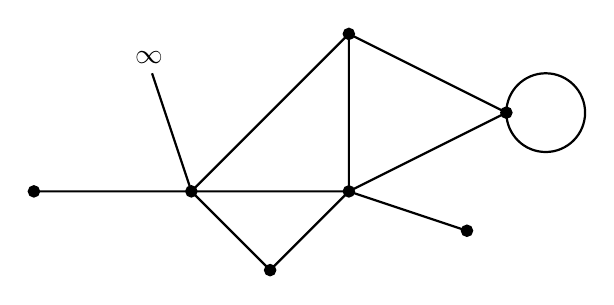
\begin{tikzpicture}[vertex/.style={draw,circle,minimum size=1.3mm,inner sep=0pt,outer sep=0pt,fill=black},scale=2, line width=0.8pt]
        \coordinate (p1) at (-0,0);
        \coordinate (p2) at (1,0);
        \coordinate (p3) at (2,0);
        \coordinate (p4) at (2,1);
        \coordinate (p5) at (1.5,-0.5);
        \coordinate (p6) at (3,0.5);
        \coordinate (p7) at (2.75,-0.25);
        \coordinate (p8) at (0.75,0.75);
        \draw (p1)--(p2)--(p3)--(p4)--(p6);
        \draw (p2)--(p4);
        \draw (p3)--(p5);
        \draw (p2)--(p5);
        \draw (p3)--(p6);
        \draw (p3)--(p7);
        \draw (p2)--(p8);
        \draw (3.25,0.5) circle (0.25);
        \node[vertex] at (p1) {};
        \node[vertex] at (p2) {};
        \node[vertex] at (p3) {};
        \node[vertex] at (p4) {};
        \node[vertex] at (p5) {};
        \node[vertex] at (p6) {};
        \node[vertex] at (p7) {};
        % \node[vertex] at (p8) {};
        \node at (0.73,0.85) {$\infty$};
      \end{tikzpicture}
    \end{figure}

    How to ``connect'' the equations at the vertices? \emph{Matching conditions.}
  \end{frame}



  \section{Quantum graphs}

  \begin{frame}
    \frametitle{Table of Contents}
    \tableofcontents[currentsection]
  \end{frame}

  \begin{frame}{Formal definition of a Quantum Graph}
    \begin{definition}
      A \emph{quantum graph} is a triple $(\Gamma, L, \text{MC})$, where
      \begin{itemize}
        \item $\Gamma$ is a \emph{metric graph},
        \item $L$ is a \emph{differential expression} defined on functions on $\Gamma$, and
        \item MC (\emph{matching conditions}) is a set of conditions relating the limit values of the functions defined on the edges of $\Gamma$.
      \end{itemize}
    \end{definition}
  \end{frame}


  \subsection{Metric graphs}

  \begin{frame}{Metric Graph}
    \begin{definition}
      A \emph{metric graph} is a tuple $(E,V)$ where:
      \begin{itemize}
        \item $E = \{e_n\}_{n=1}^N$ is a set of edges (intervals) $[x_{2n-1}, x_{2n}] \subset \mathbb{R}$.
         % called \emph{edges}, where $x_{2n-1} < x_{2n}$. At least one end-point of each interval must be finite. If both end-points are finite then the edge is called compact, otherwise it is called semi-infinite.
        \item $V = \{v_m\}_{m=1}^M$ is a partition of the set $\{x_j\}_{j=1}^{2N}$.\\Each element in $V$ is called a \emph{vertex}.
        %End-points belonging to the same vertex are identified as the same point.
      \end{itemize}
    \end{definition}
    \pause
    \begin{example}
      % \vspace{-0.2em}
      \begin{figure}
       \centering
        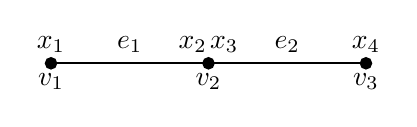
\begin{tikzpicture}[vertex/.style={draw,circle,minimum size=1.3mm,inner sep=0pt,outer sep=0pt,fill=black},scale=2, line width=0.8pt]
          \coordinate (p1) at (0,0);
          \coordinate (p2) at (1,0);
          \coordinate (p3) at (2,0);
          \draw (p1)--(p2)--(p3);
          \node[vertex] at (p1) {};
          \node[vertex] at (p2) {};
          \node[vertex] at (p3) {};
          \node[above] at (0.5,0) {$e_1$};
          \node[above] at (1.5,0) {$e_2$};
          \node[above] at (0,0) {$x_1$};
          \node[above] at (0.9,0) {$x_2$};
          \node[above] at (1.1,0) {$x_3$};
          \node[above] at (2,0) {$x_4$};
          \node[below] at (0,0) {$v_1$};
          \node[below] at (1,0) {$v_2$};
          \node[below] at (2,0) {$v_3$};
        \end{tikzpicture}
      \end{figure}
      \vspace{-2em}
      \begin{align*}
        E &= \{e_1, e_2\} = \{[x_1,x_2], [x_3,x_4]\} \\
        V &= \{v_1, v_2, v_3\} = \big\{\{x_1\}, \{x_2,x_3\}, \{x_4\}\big\}
      \end{align*}
    \end{example}
  \end{frame}

  \begin{frame}{Functions on Metric Graphs}
    \begin{definition}
      Metric graph $\Gamma$, define the Hilbert space $L_2(\Gamma)$ by
      %, the Hilbert space $L_2(\Gamma)$ and $W_2^2(\Gamma\setminus V)$ is the direct sum of the $L_2$ and $W_2^2$ spaces on each edge of $\Gamma$ respectively,
      \begin{align*}
        L_2(\Gamma) = \bigoplus_{e \in E} L_2(e), \quad\quad
        \ip{f}{g}_{L_2(\Gamma)}^2 = \int_\Gamma f(x)\overline{g}(x)\,dx.
      \end{align*}
    \end{definition}
    % \pause
    % \begin{definition}
    %   Let $\Gamma$ be a metric graph, the $L_2$ inner product and norm on $\Gamma$ is defined by
    %   \begin{align*}
    %     \ip{f}{g}_{L_2(\Gamma)} &=
    %     % \sum_{e \in E} \ip{f}{g}_{L_2(e)} =
    %     % \sum_{e \in E} \int_e f(x)\overline{g}(x)\,dx =
    %     \int_\Gamma f(x)\overline{g}(x)\,dx \\
    %     \norm{f}_{L_2(\Gamma)} &= \ip{f}{f}_{L_2(\Gamma)} = \int_{\Gamma} \abs{f(x)}^2 dx.
    %   \end{align*}
    % \end{definition}
  \end{frame}


  \subsection{Differential operators}

  \begin{frame}{Differential Expressions}
    Electric potential $q(x)$ and magnetic potential $a(x)$.

    Magnetic Schrödinger Operator
    \begin{equation*}
      L_{q,a} = \left(i\frac{d}{dx} + a(x)\right)^2 + q(x).
    \end{equation*}
    % Schrödinger operator
    % \begin{equation*}
    %   L_q \coloneqq L_{q,0} = -\frac{d^2}{dx^2} + q(x).
    % \end{equation*}
    \pause
    Laplace Operator
    \begin{equation*}
      L = L_{0,0} = -\frac{d^2}{dx^2}.
    \end{equation*}
    \pause
    The equation
    \[
      Lu = \lambda u.
    \]
  \end{frame}

  \begin{frame}{Differential Operators}
    In order to define a self-adjoint differential operator one must determine the domain of the associated differential expression.

    [Technical, see Section 2.2.2]\vspace{\baselineskip}

    Put shortly,
    \[
      0 = \langle Lu, v \rangle - \langle u, Lv \rangle.
    \]
    Implies that the energy of the system is preserved since the eigenvalues of $L$ are real, and the corresponding eigenfunctions form an orthonormal basis.
  \end{frame}


  \subsection{Matching conditions}

  % \begin{frame}{Matching Conditions: Preliminaries}
  %   % \begin{definition}
  %   %   Distinguish function values at different end-points in a vertex by defining
  %   %   \vspace{-0.5em}
  %   %   \begin{align*}
  %   %     f(x_j) =
  %   %     \begin{dcases}
  %   %       \lim_{x \to x_j^+} f(x) & j = 2n-1 \\
  %   %       \lim_{x \to x_j^-} f(x) & j = 2n.
  %   %     \end{dcases}
  %   %   \end{align*}
  %   % \end{definition}
  %   % \pause
  %   \begin{definition}
  %     The \emph{normal derivative} $\partial f(x_j)$ at an end-point $x_j$ is defined by
  %     \vspace{-0.5em}
  %     \begin{equation*}
  %       \partial f(x_j) =
  %       \begin{dcases}
  %         \lim_{x \to x_j^+}   \Dop{x} f(x) & j = 2n-1 \\
  %         \lim_{x \to x_j^-} {\color{red}\boldsymbol{-}} \Dop{x} f(x) & j = 2n.
  %       \end{dcases}
  %     \end{equation*}
  %     % Taking the derivative in the direction out from the vertex, into the edge.
  %   \end{definition}
  % \end{frame}

  \begin{frame}{Matching Conditions}
    Conditions that the functions must satisfy at each vertex so that the differential operator is self-adjoint:
    \begin{equation*}
      0 = \ip{Lu}{v} - \ip{u}{Lv} = \sum_{m=1}^{M} \sum_{x_j \in v_m} \partial u(x_j)\overline{v}(x_j) - u(x_j)\partial\overline{v}(x_j).
    \end{equation*}
    % Local matching conditions; inner sum vanishes.
    \pause
    \begin{definition}
      The \emph{standard matching conditions}, for a vertex $v$, are given by
      \begin{equation*}
        \begin{dcases}
          u(x_j) = u(x_i) \text{ for all } x_j, x_i \in v \\
          \sum_{x_j \in v} \partial u(x_j) = 0.
        \end{dcases}
      \end{equation*}
    \end{definition}
  \end{frame}


  \subsection{Scattering}

  \begin{frame}{Scattering}
    \begin{figure}
      \centering
      \begin{tikzpicture}[vertex/.style={draw,circle,minimum size=5mm,inner sep=0pt,outer sep=0pt,fill=black},scale=2, line width=0.8pt]
        \coordinate (p1) at (-2,0);
        \coordinate (p2) at (0,0);
        \draw (p1)--(p2);
        \node[vertex] at (p2) {};
        \node[above] at (0,0.15) {$\Gamma$};
        \node[above] at (-1,0) {$\overrightarrow{e^{ikx}} ~~~ R\overleftarrow{e^{-ikx}}$};
        \node at (p3) {};
      \end{tikzpicture}
    \end{figure}
    \vspace{0.5em}
    \[
      \abs{R}^2 = 1
    \]
    \pause
    \begin{figure}
      \centering
      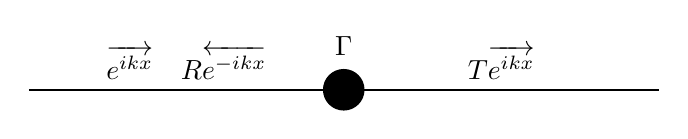
\begin{tikzpicture}[vertex/.style={draw,circle,minimum size=5mm,inner sep=0pt,outer sep=0pt,fill=black},scale=2, line width=0.8pt]
        \coordinate (p1) at (-2,0);
        \coordinate (p2) at (0,0);
        \coordinate (p3) at (2,0);
        \draw (p1)--(p2)--(p3);
        \node[vertex] at (p2) {};
        \node[above] at (0,0.15) {$\Gamma$};
        \node[above] at (-1,0) {$\overrightarrow{e^{ikx}} ~~~ R\overleftarrow{e^{-ikx}}$};
        \node[above] at (1,0) {$T\overrightarrow{e^{ikx}}$};
      \end{tikzpicture}
    \end{figure}
    \vspace{0.5em}
    \[
      \abs{R}^2 + \abs{T}^2 = 1
    \]
  \end{frame}



  \section{Snowflake graphs}

  \begin{frame}
    \frametitle{Table of Contents}
    \tableofcontents[currentsection]
  \end{frame}

  \subsection{Radial tree graphs}

  \begin{frame}{Radial Tree Graphs}
    \vspace{-0.5em}
    \begin{definition}
      A \emph{radial tree graph} $\Gamma$ is a tree where all properties depend only on the distance from the root vertex.
      \begin{itemize}
        \item The $n$:th \emph{generation} is the set of all edges being $n-1$ edges away from the root vertex.
        \item The \emph{branching number} $b_n$ of the $n$:th generation is the number of edges connected to each edge in generation $n-1$.
      \end{itemize}
    \end{definition}
    \vspace{-0.8em}
    \begin{figure}
      \centering
      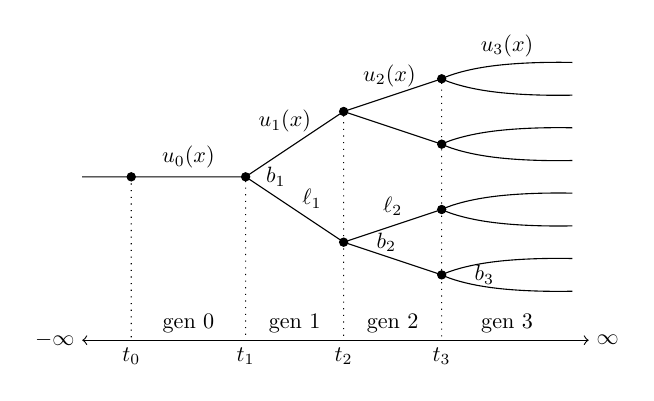
\begin{tikzpicture}[vertex/.style={draw,circle,minimum size=1.3mm,inner sep=0pt,outer sep=0pt,fill=black},scale=0.83,every node/.style={scale=0.8}]
        \path
          (0.25,0) node[vertex] (0)   {}
          (2,0)    node[vertex] (p0)  {}
          (3.5,1)  node[vertex] (p11) {}
          (3.5,-1) node[vertex] (p12) {}
          (5,1.5)  node[vertex] (p21) {}
          (5,0.5)  node[vertex] (p22) {}
          (5,-0.5) node[vertex] (p23) {}
          (5,-1.5) node[vertex] (p24) {};
        \node[right=0.2cm] at (p0) {$b_1$};
        \node[right=0.4cm] at (p12) {$b_2$};
        \node[right=0.4cm] at (p24) {$b_3$};
        \node[above right] at (2.75,-0.6) {$\ell_1$};
        \node at (4.25,-0.45) {$\ell_2$};
        \node at (1.125,0.3) {$u_0(x)$};
        \node at (2.6,0.85) {$u_1(x)$};
        \node at (4.2,1.55) {$u_2(x)$};
        \node at (6,2) {$u_3(x)$};
        \draw
          (-0.5,0) -- (0)
          (0)   -- (p0)
          (p0)  -- (p11)
          (p0)  -- (p12)
          (p11) -- (p21)
          (p11) -- (p22)
          (p12) -- (p23)
          (p12) -- (p24);
        \draw plot [smooth,tension=1] coordinates{(p21) (5.8,1.7) (7,1.75)};
        \draw plot [smooth,tension=1] coordinates{(p21) (5.8,1.3) (7,1.25)};
        \draw plot [smooth,tension=1] coordinates{(p22) (5.8,0.7) (7,0.75)};
        \draw plot [smooth,tension=1] coordinates{(p22) (5.8,0.3) (7,0.25)};
        \draw plot [smooth,tension=1] coordinates{(p23) (5.8,-0.7) (7,-0.75)};
        \draw plot [smooth,tension=1] coordinates{(p23) (5.8,-0.3) (7,-0.25)};
        \draw plot [smooth,tension=1] coordinates{(p24) (5.8,-1.7) (7,-1.75)};
        \draw plot [smooth,tension=1] coordinates{(p24) (5.8,-1.3) (7,-1.25)};
        \draw[dotted]
          (0.25,0) -- (0.25,-2.5)
          (p0)     -- (2,-2.5)
          (p11)    -- (3.5,-2.5)
          (p21)    -- (5,-2.5);
        \draw[<->] (-0.5,-2.5) -- (7.25,-2.5);
        \node[below] (t0) at (0.25,-2.5) {$t_0$};
        \node[below] (t1) at (2,-2.5) {$t_1$};
        \node[below] (t2) at (3.5,-2.5) {$t_2$};
        \node[below] (t3) at (5,-2.5) {$t_3$};
        \node[left]  (-infty) at (-0.5,-2.5) {$-\infty$};
        \node[right] (intfy) at (7.25,-2.5) {$\infty$};
        \node[above] at (1.125,-2.5) {gen 0};
        \node[above] at (2.75,-2.5) {gen 1};
        \node[above] at (4.25,-2.5) {gen 2};
        \node[above] at (6,-2.5) {gen 3};
      \end{tikzpicture}
    \end{figure}
  \end{frame}

  \begin{frame}{Scattering from 2-generation radial tree graph}
    \begin{theorem}
      Let $\Gamma$ be a 2-gen radial tree with standard matching conditions. The reflection coefficient and reflection probability are, respectively, given by
      \vspace{-0.5em}
      \begin{align*}
        R(k) &= -\frac{(b_1-1) (b_2+1)+(b_1+1) (b_2-1) e^{2 i k \ell_1}}{(b_1+1) (b_2+1)+(b_1-1) (b_2-1) e^{2 i k \ell_1}}.
      \end{align*}
    \end{theorem}
  \end{frame}

  \begin{frame}{Scattering from 2-generation radial tree graph}
    \begin{proof}
      Find the eigenfunctions on each edge
      \begin{equation*}
        u(x) = \begin{cases}
             e^{ikx} + Re^{-ikx}   & \text{generation 0} \\
          Ae^{ikx} + Be^{-ikx} & \text{generation 1} \\
          Te^{ikx}                 & \text{generation 2}.
        \end{cases}
      \end{equation*}
      Write down the equations given by the standard matching conditions
      \begin{align*}
        & \begin{cases}
          1+R = A+B \\
          -ik(1-R) + b_1 ik(A-B) = 0
        \end{cases} \\
        & \begin{cases}
          Ae^{ik\ell_1} + Be^{-ik\ell_1} = Te^{ik\ell_1} \\
          -ik(Ae^{ik\ell_1}-Be^{-ik\ell_1}) + b_2 ikTe^{ik\ell_1} = 0.
        \end{cases}
      \end{align*}
      Solve for $R$.
    \end{proof}
  \end{frame}

  \begin{frame}{Scattering from 2-generation radial tree graph}
    \vspace{-0.5em}
    \begin{theorem}
      Let $\Gamma$ be a 2-gen radial tree with standard matching conditions. The reflection coefficient and reflection probability are, respectively, given by
      \vspace{-0.5em}
      \begin{align*}
        R(k) &= -\frac{(b_1-1) (b_2+1)+(b_1+1) (b_2-1) e^{2 i k \ell_1}}{(b_1+1) (b_2+1)+(b_1-1) (b_2-1) e^{2 i k \ell_1}}, \\
        \abs{R(k)}^2 &= \frac{(b_1-b_2)^2 \sin ^2(k \ell_1)+(b_1 b_2-1)^2 \cos ^2(k \ell_1)}{(b_1+b_2)^2 \sin ^2(k \ell_1)+(b_1 b_2+1)^2 \cos ^2(k \ell_1)}.
      \end{align*}
    \end{theorem}
    \vspace{-1em}
    \pause
    \begin{corollary}
      \begin{itemize}
        \item $R(0) = \frac{2}{b_1b_2+1} - 1$, low-energy waves do not ``see'' the middle edges.
        \item Let $\widehat{\Gamma}$ be $\Gamma$ with $b_1$ and $b_2$ interchanged, since $\abs{R(k)}^2$ is invariant when interchanging $b_1$ and $b_2$, the graphs $\widehat{\Gamma}$ and $\Gamma$ cannot be distinguished by measuring the reflection probability from the root of the graphs.
        \item Zero reflection is possible only when $b_1=b_2$.
      \end{itemize}
    \end{corollary}
  \end{frame}

  \begin{frame}{Scattering from 2-generation radial tree}
    \begin{figure}[h]
      \begin{subfigure}[t]{0.35\textwidth}
        \includegraphics[width=1\textwidth]{../latex/img/2gen_reflection_l=1_b1=3_b2=7}
        \caption{$b_1=7, b_2=3$}
      \end{subfigure}
      \begin{subfigure}[t]{0.35\textwidth}
        \includegraphics[width=1\textwidth]{../latex/img/2gen_reflection_l=1_b1=b2=4}
        \caption{$b_1=b_2=4$}
      \end{subfigure}
      \\
      \begin{subfigure}[t]{0.35\textwidth}
        \includegraphics[width=1\textwidth]{../latex/img/2gen_reflection_l=1_b1=500_b2=10}
        \caption{$b_1=500, b_2=10$}
      \end{subfigure}
      \begin{subfigure}[t]{0.35\textwidth}
        \includegraphics[width=1\textwidth]{../latex/img/2gen_reflection_l=1_b1=100_b2=100}
        \caption{$b_1=b_2=100$}
      \end{subfigure}
      \vspace{-0.3em}
      \caption{Reflection $\abs{R}^2$ from 2 generation radial quantum tree graph with inner edge length $\ell_1=1$ and varying branching numbers $b_1$ and $b_2$.}
      \label{fig: 2 gen reflection}
    \end{figure}
  \end{frame}


  \subsection{Defining the snowflake}

  \begin{frame}[t]{Defining the snowflake graph}
    \vspace{-0.5em}
    \begin{definition}
      A \emph{quantum snowflake} graph $\Gamma$ is a radial quantum tree graph with infinite number of generations, all with branching number $m$. Furthermore, the length of all edges in generation $k$ is $\ell\beta^k$ where $\ell$ and $\beta$ are constant.
    \end{definition}
    % \pause
    \only<1-1>{\begin{figure}
      \centering
      \includegraphics[width=0.6\textwidth]{../latex/img/{snowflake_4_0.35_7_4_0.5}.pdf}
    \end{figure}}
    \only<2-2>{\begin{itemize}
      \item If $0 < \beta < 1$ the graph has finite depth $\sum_{k=0}^{\infty} \ell\beta^k = \frac{\ell}{1-\beta}$.
      % \item If the number of generations is finite and all edges are finite, then the entire wave necessarily gets reflected, $\abs{R} \equiv 1$.
      \item Waves disperse in the infinite structure.
      % \item We shall only consider snowflake graphs with standard matching conditions.
    \end{itemize}}
  \end{frame}

  \begin{frame}{Illustration of notation}
    Index edges by $e_{j_1,j_2,\ldots,j_n} = e_{\vec{j}}$, similarly vertex $v_{\vec{j}}$ is given by the right end-point of $e_{\vec{j}}$.
    \vspace{-1.7em}
    \begin{figure}
      \centering
      \includegraphics[height=0.8\textheight]{../latex/img/snowflake_2.tikz}
      \caption{A snowflake with only 2 generations, branching number $m=4$ and $\beta < 1$, illustrating our notation.}
    \end{figure}
  \end{frame}


  \subsection{Rotational symmetries}

  \begin{frame}{Rotation Operator}
    For $\vec{k} = (k_1, k_2, \ldots, k_n)$ and $\vec{j} = (j_1, j_2, \ldots, j_m)$ we define the rotation $R_{\vec{k}}$ as the cyclic permutation of edges
    \[
      R_{\vec{k}} e_{\vec{j}} =
      \begin{cases}
        e_{j_1, j_2, \ldots, j_m}, & n > m \\
        e_{j_1, j_2, \ldots, j_{n-1}, j_n + 1, j_{n+1}, \ldots, j_m}, & n \le m.
      \end{cases}
    \]
    Cyclic notation $e_{j_1, \ldots, j_k+m, \ldots, j_n} = e_{j_1, \ldots, j_k, \ldots, j_n}$.
  \end{frame}

  \begin{frame}{Rotational symmetries on $\Gamma_1$}
    Because of the self-similarity of $\Gamma$, it suffices to consider a 1-generation sub-graph $\Gamma_1$ to study the rotational symmetries.
    \vspace{-0.5em}
    \begin{figure}
      \centering
      \includegraphics[width=0.4\textwidth]{../latex/img/star_graph_2.tikz}
    \end{figure}
    \vspace{-2em}
    Only one rotation operator $R=R_0$
    \begin{align*}
      \begin{cases}
        R e_j = e_{j+1}, & j = 1, 2, \ldots, m \\
        R e_0 = e_{0}
      \end{cases} &&
      \begin{cases}
        (R f)_{j} = f_{j+1}, & j = 1, 2, \ldots, m \\
        (R f)_{0} = f_{0}.
      \end{cases}
    \end{align*}
  \end{frame}

  \begin{frame}{Rotation-eigenfunctions}
    \begin{itemize}
      \item In general $Rf \ne f$, but $R^m f = f$, hence $R^m$ has eigenvalue $1$.
      \item $R$ has eigenvalues $z^n, 0 \le n \le m-1$ where $z = e^{i2\pi/m}$.
      \item Let $f^n$ be the corresponding eigenfunction,
      \[
        Rf^n = z^nf^n.
      \]
    \end{itemize}
    \pause
    \begin{lemma}
      Every eigenfunction $f^n$ of $R$, except $f^0$, vanishes everywhere on the root edge $e_0$.
    \end{lemma}
    \begin{proof}
      In generation 0 rotations do nothing, hence
      $R f^n_0 = f^n_0 = z^n f_0$, implying $f^n_0 \equiv 0$ for $1 \le n \le m-1$.
    \end{proof}
  \end{frame}

  \begin{frame}{Quasi rotation invariant component}
    \begin{definition}
      The $n$-th quasi rotation invariant component $f^n$ of a function $f$ on $\Gamma_1$ is defined by
      \begin{equation*}
          f^n_j = \frac{1}{m} \sum_{k=0}^{m-1} z^{-nk} f_{j+k}, \quad j = 1, 2, \ldots, m
      \end{equation*}
      on the first generation, where $z=e^{\frac{2\pi}{m}i}$, and on the root edge $e_0$ it is defined by
      \[
        \begin{cases}
          f^n_0 = 0, \quad 0 \le n \le m-1 \\
          f^0_0 = f_0
        \end{cases}
      \]
      where $f_j$ denotes the restriction of $f$ to the edge $e_j$.
    \end{definition}
    \begin{itemize}
      \item Generalization of even and odd functions.
      \item There are $m$ such components, since $f^{n+m} = f^{n}$, because $z^{-(n+m)k} = z^{-nk}(z^m)^{-k}$ and $z^m=1$.
    \end{itemize}
  \end{frame}

  \begin{frame}{The notation is consistent}
    \begin{theorem}
      Let $f^n$ for $n = 1, 2, \ldots, m-1$ be the quasi rotation invariant components of an arbitrary functions $f$ defined on the graph. Then
      \begin{enumerate}[(a)]
        \item $f^n$ is an eigenfunction of $R$ with the corresponding eigenvalue $z^n$, % Conversely, every eigenfunction of $R$ is a quasi rotation invariant component of some function.
        \item $f$ is the sum of its quasi rotation invariant components.%: $f = \displaystyle\sum_{n=0}^{m-1} f^n$.
      \end{enumerate}
    \end{theorem}
    \pause
    \begin{corollary}
      By repeated rotations we have
      \[
        f^n_j = z f^n_{j-1} = \ldots = z^{n(j-1)} f^n_1, \quad j = 1, 2, \ldots, m,
      \]
      together with {\normalfont(b)} this shows that $f$ on one entire generation can be reconstructed from the values of $f^n$ on just one edge in the same generation.
    \end{corollary}
  \end{frame}


  \subsection{Collapsing the snowflake}

  \begin{frame}{Collapsing the snowflake}
    \begin{definition}
      Quantum snowflake $\Gamma$ with edges $e_{j_1,j_2,\ldots}$ define collapsed line-graph $\widetilde{\Gamma}$ by
      \begin{align*}
        \widetilde{\Gamma} &= e_0 \cup e_1 \cup e_{11} \cup e_{111} \cup \ldots.
      \end{align*}
    \end{definition}
    \pause
    \begin{itemize}
      \item Study $\Gamma$ via $\widetilde{\Gamma}$.
      \item Matching conditions on $\widetilde{\Gamma}$ so that $\Gamma$ and $\widetilde{\Gamma}$ have equal reflection.
      \item Self-similarity $\to$ suffices to consider $\Gamma_1$ and $\widetilde{\Gamma}_1 = e_0 \cup e_1$.
    \end{itemize}
  \end{frame}

  \begin{frame}{Transforming $L_2(\Gamma_1) \to L_2(\widetilde{\Gamma}_1)$}
    \begin{theorem}
      Let $f^n$ and $g^m$ be eigenfunctions of $R$, i.e.\ $R f^n = z^n f^n$ and $R g^m = z^m g^m$, then
      $f^n$ and $g^m$ are orthogonal for $n \ne m$ and $\ip{f^n}{g^n} = \ip{f^n_0}{g^n_0} + m \ip{f^n_1}{g^m_1}$, where $f^n_0$ is non-zero only for $n=0$.
    \end{theorem}
    \pause
    Hence
    \vspace{-1em}
    \begin{align*}
      \norm{f}_{L_2(\Gamma_1)}^2 &= \norm{f_0}^2 + m\norm{f_1}^2 \\
      \norm{f}_{L_2(\widetilde{\Gamma}_1)}^2 &= \norm{f_0}^2 + \norm{f_1}^2.
    \end{align*}
    \pause
    There exists a unitary transformation, as illustrated, hence the graphs are isospectral. We cut off the redundant edges to get $\widetilde{\Gamma}_1$.
    \begin{figure}
      \centering
      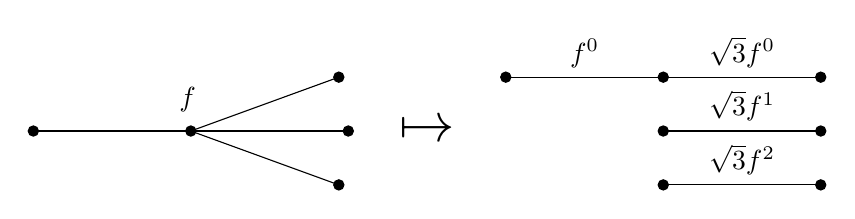
\begin{tikzpicture}[vertex/.style={draw,circle,minimum size=1.3mm,inner sep=0pt,outer sep=0pt,fill=black},scale=2]

        \draw (-1, 0) -- (0, 0);
        \node[vertex] at (-1, 0) {};
        \node[vertex] at (0, 0) {};

        \pgfmathsetmacro{\v}{20}

        \draw (0, 0) -- ({cos(\v)}, {sin(\v)});
        \node[vertex] at ({cos(\v)}, {sin(\v)}) {};

        \draw (0, 0) -- (1, 0);
        \node[vertex] at (1, 0) {};

        \draw (0, 0) -- ({cos(-\v)}, {sin(-\v)});
        \node[vertex] at ({cos(-\v)}, {sin(-\v)}) {};

        \draw (2, {sin(\v)}) -- (4, {sin(\v)});
        \node[vertex] at (2, {sin(\v)}) {};
        \node[vertex] at (3, {sin(\v)}) {};
        \node[vertex] at (4, {sin(\v)}) {};

        \node at (-0.02, 0.2) {$f$};

        \node[scale=2] at (1.5, 0) {$\mapsto$};

        \draw (3, 0) -- (4, 0);
        \node[vertex] at (3, 0) {};
        \node[vertex] at (4, 0) {};

        \draw (3, {sin(-\v)}) -- (4, {sin(-\v)});
        \node[vertex] at (3, {sin(-\v)}) {};
        \node[vertex] at (4, {sin(-\v)}) {};

        \node[above] at (2.5, {sin(\v)}) {$f^0$};
        \node[above] at (3.5, {sin(\v)}) {$\sqrt{3} f^0$};
        \node[above] at (3.5, 0) {$\sqrt{3} f^1$};
        \node[above] at (3.5, {sin(-\v)}) {$\sqrt{3} f^2$};
      \end{tikzpicture}
    \end{figure}
  \end{frame}


  \subsection[Collapsed MC]{Collapsed matching conditions}

  \begin{frame}{Matching Conditions on the Collapsed Snowflake}
    \begin{theorem}
      Quantum snowflake $\Gamma$, branching number $m$, standard matching conditions. Corresponding collapsed graph $\widetilde{\Gamma}$. Then $\Gamma$ and $\widetilde{\Gamma}$ have equal reflection if the matching conditions for $\widetilde{\Gamma}$ are chosen as
      \begin{equation*}
        \begin{dcases}
          f_{n+1}(v_{n+1}) = \sqrt{m} f_n(v_{n+1}) \\
          f'_{n+1}(v_{n+1}) = \frac{1}{\sqrt{m}} f'_n(v_{n+1})
        \end{dcases}
      \end{equation*}
      for every vertex $v_1,v_2,\ldots$ in $\widetilde{\Gamma}$.
    \end{theorem}
  \end{frame}


  \subsection{Snowflake scattering}

  \begin{frame}{Scattering in the Snowflake Graph}
    Problem reduced to finding reflection of
    \begin{figure}
      \centering
      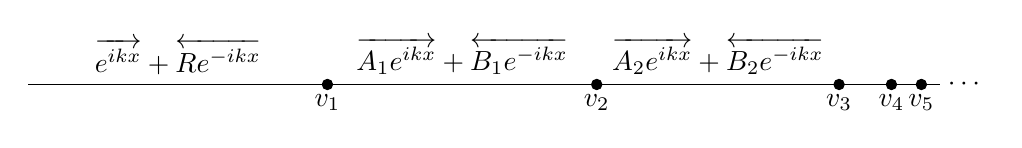
\begin{tikzpicture}[vertex/.style={draw,circle,minimum size=1.3mm,inner sep=0pt,outer sep=0pt,fill=black}, scale=0.95]
        \pgfmathsetmacro{\q}{0.9}
        \draw (-4,0) -- node[above] {$\overrightarrow{e^{ikx}} + \overleftarrow{Re^{-ikx}}$} (0,0) --
          node[above] {$\overrightarrow{A_1 e^{ikx}} + \overleftarrow{B_1 e^{-ikx}}$} ({4*\q^1},0) --
          node[above] {$\overrightarrow{A_2 e^{ikx}} + \overleftarrow{B_2 e^{-ikx}}$} ({4*\q^1+4*\q^2},0) --
          node[above] {} ({4*\q^1+4*\q^2+1.35},0);
        \node[vertex] at (0,0) {};
        \node[below] at (0,0) {$v_1$};
        \node[vertex] at ({4*\q^1},0) {};
        \node[below] at ({4*\q^1},0) {$v_2$};
        \node[vertex] at ({4*\q^1+4*\q^2},0) {};
        \node[below] at ({4*\q^1+4*\q^2},0) {$v_3$};
        \node[vertex] at ({4*\q^1+4*\q^2+0.7},0) {};
        \node[below] at ({4*\q^1+4*\q^2+0.7},0) {$v_4$};
        \node[vertex] at ({4*\q^1+4*\q^2+1.1},0) {};
        \node[below] at ({4*\q^1+4*\q^2+1.1},0) {$v_5$};
        % \node[vertex] at ({4*\q^1+4*\q^2+1.5},0) {};
        \node[] at ({4*\q^1+4*\q^2+1.7},0) {$\cdots$};
      \end{tikzpicture}
    \end{figure}
    \begin{align*}
      \begin{dcases}
        A_n e^{ik\beta^n} + B_n e^{ik\beta^n} = \frac{1}{\sqrt{m}} \big( A_{n+1} + B_{n+1} \big) \\
        A_n e^{ik\beta^n} - B_n e^{ik\beta^n} = \sqrt{m} \big( A_{n+1} - B_{n+1} \big).
      \end{dcases}
    \end{align*}
    Can no longer use self-similarity, reflection contribution from all edges; occurrence of $\beta^n \ne \beta^{n+1}$ in the $n$-th equation.
  \end{frame}

  \begin{frame}{Step by Step: First step}
    Notation: $S_{ij}$, wave scattered towards direction $i$ from direction $j$. $i,j=\text{left},\text{right}$.
    \begin{figure}
      \centering
      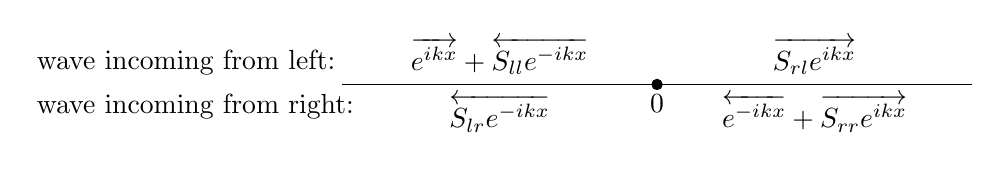
\begin{tikzpicture}[vertex/.style={draw,circle,minimum size=1.3mm,inner sep=0pt,outer sep=0pt,fill=black}, scale=1]
        \draw (-4,0) -- (0,0) -- (4,0);
        \node[vertex] at (0,0) {};
        \node[below] at (0,0) {$0$};

        \node[above] at (-2,0) {$\overrightarrow{e^{ikx}} + \overleftarrow{S_{ll} e^{-ikx}}$};
        \node[above] at (2,0)  {$\overrightarrow{S_{rl} e^{ikx}}$};

        \node[below] at (-2,0) {$\overleftarrow{S_{lr} e^{-ikx}}$};
        \node[below] at (2,0)  {$\overleftarrow{e^{-ikx}} + \overrightarrow{S_{rr} e^{ikx}}$};

        \node[above right] at (-8,0) {wave incoming from left:};
        \node[below right] at (-8,0) {wave incoming from right:};
      \end{tikzpicture}
    \end{figure}
    \vspace{-1em}\pause
    \begin{align*}
      \text{wave incoming from left:} & \begin{dcases}
        1 + S_{ll} = \frac{1}{\sqrt{m}} S_{rl} \\
        1 - S_{ll} = \sqrt{m} S_{rl}
      \end{dcases}
      && \!\!\!\!\!\!\!\!\implies \begin{dcases}
        S_{ll} = \frac{1-m}{1+m} \\
        S_{rl} = \frac{2\sqrt{m}}{1+m}
      \end{dcases}
      \\
      \text{wave incoming from right:} & \begin{dcases}
        S_{lr} = \frac{1}{\sqrt{m}} \big( 1 + S_{rr} \big) \\
        -S_{lr} = \sqrt{m} \big( - 1 + S_{rr} \big)
      \end{dcases}
      && \!\!\!\!\!\!\!\!\implies \begin{dcases}
        S_{rr} = -\frac{1-m}{1+m} \\
        S_{lr} = \frac{2\sqrt{m}}{m+1}.
      \end{dcases}
    \end{align*}
    $S_{rr} = - S_{ll}$ and $S_{rl} = S_{lr}$.
  \end{frame}

  \begin{frame}{Step by Step: Second step}
    \begin{figure}
      \centering
      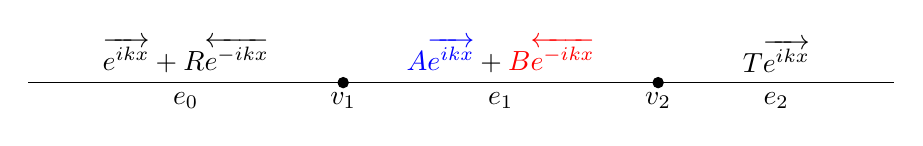
\begin{tikzpicture}[vertex/.style={draw,circle,minimum size=1.3mm,inner sep=0pt,outer sep=0pt,fill=black}, scale=1]
        \draw (-4,0) -- (0,0) -- (4,0) -- (7,0);

        \node[vertex] at (0,0) {};
        \node[below] at (0,0) {$v_1$};

        \node[vertex] at (4,0) {};
        \node[below] at (4,0) {$v_2$};

        \node[above] at (-2,0) {$\overrightarrow{e^{ikx}} + R \overleftarrow{e^{-ikx}}$};
        \node[below] at (-2,0) {$e_0$};
        \node[above] at (2,0) {${\color{blue}A \overrightarrow{e^{ikx}}} + {\color{red}B \overleftarrow{e^{-ikx}}}$};
        \node[below] at (2,0) {$e_1$};
        \node[above] at (5.5,0) {$T \overrightarrow{e^{ikx}}$};
        \node[below] at (5.5,0) {$e_2$};
      \end{tikzpicture}
    \end{figure}
    Total wave on $e_1$:
    \begin{equation*}
      \begin{aligned}
        & {\color{blue}S_{rl} \overrightarrow{e^{ik(x-v_1)}}} + \\
        & {\color{red}S_{rl} e^{ik(v_2-v_1)} S_{ll} \overleftarrow{e^{-ik(x-v_2)}}} + \\
        & {\color{blue}S_{rl} e^{ik(v_2-v_1)} S_{ll} e^{-ik(v_1-v_2)} S_{rr} \overrightarrow{e^{ik(x-v_1)}}} + \\
        & {\color{red}S_{rl} e^{ik(v_2-v_1)} S_{ll} e^{-ik(v_1-v_2)} S_{rr} e^{ik(v_2-v_1)} S_{ll} \overleftarrow{e^{-ik(x-v_2)}}} + \\
        & {\color{blue}S_{rl} e^{ik(v_2-v_1)} S_{ll} e^{-ik(v_1-v_2)} S_{rr} e^{ik(v_2-v_1)} S_{ll} e^{-ik(v_1-v_2)} S_{rr} \overrightarrow{e^{ik(x-v_2)}}} + \ldots
        % & S_{rl} e^{ik(v_2-v_1)} S_{ll} e^{-ik(v_1-v_2)} S_{rr} e^{ik(v_2-v_1)} S_{ll} e^{-ik(v_1-v_2)} S_{rr} e^{ik(v_2-v_1)} S_{ll} \overleftarrow{e^{-ik(x-v_2)}} + \ldots
        % & \vdots
      \end{aligned}
    \end{equation*}
  \end{frame}

  \begin{frame}{Step by Step: Second step}
    Converging geometric series for coefficients $R, A, B, T$.
    \vspace{1em}
    \begin{align*}
      A &= S_{rl} \left(1 + e^{2ik\ell_1} S_{ll} S_{rr} + \left(e^{2ik\ell_1} S_{ll} S_{rr}\right)^2 + \ldots \right) \\[1.5em]
      &= \frac{S_{rl}}{1-e^{2ik\ell_1}S_{ll}S_{rr}}
      % B \overleftarrow{e^{-ik(x-v_1)}}
      % &= S_{rl} S_{ll} e^{ik\ell_1} e^{-ik(x-v_2)} \left(1 + e^{2ik\ell_1} S_{rr} S_{ll} +  \left(e^{2ik\ell_1} S_{rr} S_{ll}\right)^2 + \ldots \right) \overleftarrow{e^{-ik(x-v_2)}} \\
      % &= \frac{e^{ik\ell_1} S_{rl} S_{ll}}{1 - e^{2ik\ell_1} S_{ll} S_{rr}} \overleftarrow{e^{-ik(x-v_2)}} \\
      % T \overrightarrow{e^{ik(x-v_2)}}
      % &= S_{rl} e^{ik\ell_1} \left( 1 + e^{2ik\ell_1} S_{ll} S_{rr} + \left(e^{2ik\ell_1} S_{ll} S_{rr}\right)^2 + \ldots \right) S_{rl} \overrightarrow{e^{ik(x-v_2)}} \\
      % &= \frac{e^{ik\ell_1} S_{rl}^2}{1 - e^{2ik\ell_1} S_{ll} S_{rr}} \overrightarrow{e^{ik(x-v_2)}} \\
      % R \overleftarrow{e^{-ik(x-v_1)}}
      % &= S_{ll} \overleftarrow{e^{-ik(x-v_1)}} + B e^{-ikv_1} S_{lr} \overleftarrow{e^{-ik(x-v_1)}} \\
      % &= \left( S_{ll} + \frac{e^{2ik\ell_1} S_{rl} S_{ll} S_{lr}}{1 - e^{2ik\ell_1} S_{ll} S_{rr}} \right) \overleftarrow{e^{-ik(x-v_1)}}
    \end{align*}
  \end{frame}


  \subsection{Merging vertices}

  \begin{frame}{Merging vertices}
    \begin{figure}
      \centering
      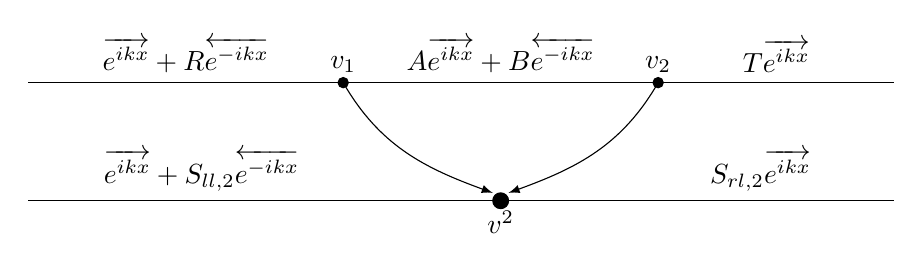
\begin{tikzpicture}[vertex/.style={draw,circle,minimum size=1.3mm,inner sep=0pt,outer sep=0pt,fill=black}, scale=1]
        \draw (-4,0) -- (7,0);

        \node[vertex] at (0,0) {};
        \node[above] at (0,0) {$v_1$};

        \node[vertex] at (4,0) {};
        \node[above] at (4,0) {$v_2$};

        \node[above] at (-2,0) {$\overrightarrow{e^{ikx}} + R \overleftarrow{e^{-ikx}}$};
        \node[above] at (2,0) {$A \overrightarrow{e^{ikx}} + B \overleftarrow{e^{-ikx}}$};
        \node[above] at (5.5,0) {$T \overrightarrow{e^{ikx}}$};

        \pgfmathsetmacro{\y}{-1.5}
        \draw (-4,\y) -- (7,\y);

        \node[vertex,style={minimum size=2mm}] at (2,\y) {};
        \node[below] at (2,\y) {$v^2$};

        \draw[-latex] (0,0) to[out=300,in=160,looseness=1] (1.9,{\y+0.1});
        \draw[-latex] (4,0) to[out=240,in=20 ,looseness=1] (2.1,{\y+0.1});

        % \node[above] at (-1,\y) {$\overrightarrow{e^{ikx}} + R \overleftarrow{e^{-ikx}}$};
        \node[above] at (-1.8,\y) {$\overrightarrow{e^{ikx}} + S_{ll,2} \overleftarrow{e^{-ikx}}$};
        % \node[above] at (4.5,\y) {$T \overrightarrow{e^{ikx}}$};
        \node[above] at (5.3,\y) {$S_{rl,2} \overrightarrow{e^{ikx}}$};
      \end{tikzpicture}
    \end{figure}
    \pause
    \begin{align*}
      S_{ll,2} &= S_{ll} + \frac{e^{2ik\ell_1} S_{rl} S_{ll} S_{lr}}{1 - e^{2ik\ell_1} S_{ll} S_{rr}} \\
      \color{gray}S_{rl,2} & \color{gray}= S_{rl,2}\frac{e^{ik\ell_1} S_{rl}^2}{1 - e^{2ik\ell_1} S_{ll} S_{rr}} \\
      \color{gray}S_{rr,2} & \color{gray}= S_{rl,2}S_{rr} + \frac{e^{2ik\ell_1} S_{lr} S_{rr} S_{rl}}{1 - e^{2ik\ell_1} S_{rr} S_{ll}} \\
      \color{gray}S_{lr,2} & \color{gray}= S_{rl,2}\frac{e^{ik\ell_1} S_{lr}^2}{1 - e^{2ik\ell_1} S_{rr} S_{ll}}
    \end{align*}

  \end{frame}


  \subsection{Recursion}

  \begin{frame}{Recursive expression for reflection from $n$ generations}
    \begin{figure}
      \centering
      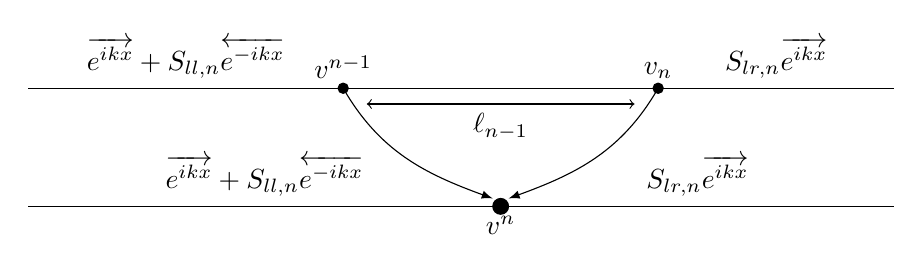
\begin{tikzpicture}[vertex/.style={draw,circle,minimum size=1.3mm,inner sep=0pt,outer sep=0pt,fill=black}, scale=1]
        \draw (-4,0) -- (7,0);

        \node[vertex] at (0,0) {};
        \node[above] at (0,0) {$v^{n-1}$};

        \node[vertex] at (4,0) {};
        \node[above] at (4,0) {$v_n$};

        \node[above] at (-2,0) {$\overrightarrow{e^{ikx}} + S_{ll,n} \overleftarrow{e^{-ikx}}$};
        \node[above] at (5.5,0) {$S_{lr,n} \overrightarrow{e^{ikx}}$};

        \pgfmathsetmacro{\y}{-1.5}
        \draw (-4,\y) -- (7,\y);

        \node[vertex,style={minimum size=2mm}] at (2,\y) {};
        \node[below] at (2,\y) {$v^n$};

        \draw[<->] ({0+0.3},-0.2) to ({4-0.3},-0.2);
        \node[below] at (2,-0.2) {$\ell_{n-1}$};

        \draw[-latex] (0,0) to[out=300,in=160,looseness=1] (1.9,{\y+0.1});
        \draw[-latex] (4,0) to[out=240,in=20 ,looseness=1] (2.1,{\y+0.1});

        \node[above] at (-1,\y) {$\overrightarrow{e^{ikx}} + S_{ll,n} \overleftarrow{e^{-ikx}}$};
        \node[above] at (4.5,\y) {$S_{lr,n} \overrightarrow{e^{ikx}}$};
      \end{tikzpicture}
    \end{figure}
  \end{frame}

  \begin{frame}{Recursive expression for reflection from $n$ generations}
    \begin{theorem}
      Let $\Gamma$ be a quantum snowflake graph with $n+1$ generations, branching number $m$ and edge length $\ell_j = \ell\beta^j$ in generation $j$. Then the total reflection $R_{n+1}(k) = S_{ll,n+1}(k)$ is given by the recursion formula
      \begin{align*}
        \left\lbrace\!
        \begin{aligned}
          S_{ll,1} &= \frac{1-m}{1+m} \\
          S_{rl,1} &= \frac{2\sqrt{m}}{1+m} \\
          S_{rr,1} &= -S_{ll,1} \\
          S_{lr,1} &= S_{rl,1}
        \end{aligned}\right.
        &&
        \left\lbrace\!
        \begin{aligned}
          S_{ll,n+1} &= S_{ll,n} + \frac{e^{2ik\ell_n} S_{rl,n} S_{ll,1} S_{lr,n}}{1 - e^{2ik\ell_n} S_{rr,n} S_{ll,1}} \\
          S_{rl,n+1} &= \frac{e^{ik\ell_n} S_{rl,n} S_{rl,1}}{1 - e^{2ik\ell_n} S_{ll,1} S_{rr,n}} \\
          S_{rr,n+1} &= S_{rr,1} + \frac{e^{2ik\ell_n} S_{lr,1} S_{rr,n} S_{rl,1}}{1 - e^{2ik\ell_n} S_{ll,1} S_{rr,n}} \\
          S_{lr,n+1} &= \frac{e^{ik\ell_n} S_{lr,1}S_{lr,n}}{1 - e^{2ik\ell_n} S_{rr,n} S_{ll,1}}
        \end{aligned}\right.
      \end{align*}
    \end{theorem}
  \end{frame}

  % \begin{frame}{Recursive expression for reflection from $n$ generations}
  %   \begin{corollary}
  %     Let $\Gamma$ and $\Gamma'$ be two quantum snowflake graphs with equal edge length and branching number $m$ and $m'$, respectively. If $m > m'$ then
  %     \[
  %       \abs{R_m(k)}^2 \ge \abs{R_{m'}(k)}^2
  %     \]
  %     with equality only for $k$ satisfying $\abs{R_m(k)}^2 = 0$ or $\abs{R_m(k)}^2 = 1$.
  %   \end{corollary}
  % \end{frame}

  \begin{frame}{Non-periodicity and irregularity}{}
    {\footnotesize
    \begin{equation*}
      S_{3,ll} = -\frac{(m-1) \left((m-1)^2 e^{2 i \beta^3 k \ell}+(m+1)^2 e^{2 i \beta^2 k \ell}+(m+1)^2 e^{2 i \beta^2 (\beta+1) k
         \ell}+(m+1)^2\right)}{(m+1) \left((m-1)^2 e^{2 i \beta^3 k \ell}+(m-1)^2 e^{2 i \beta^2 k \ell}+(m-1)^2 e^{2 i \beta^2
         (\beta+1) k \ell}+(m+1)^2\right)}
    \end{equation*}}
    \vspace{1em}
    \pause
    \[
      R(k;m,\beta) = \lim_{n\to\infty} S_{ll,n}(k;m,\beta)
      \vspace{1em}
    \]
    Closed-form expression? The seemingly irregular behavior makes this very difficult.
  \end{frame}

  \begin{frame}{Plots of $\abs{R}^2$ for Finite Snowflakes}
    \begin{figure}
      \begin{subfigure}[t]{\textwidth}
        \centering
        \includegraphics[width=0.7\textwidth]{../latex/img/reflection_n=6_m=2_l=1_b=07_kmax=80}
        \caption{$n=6, m=2, \ell=1, \beta=0.7$}
      \end{subfigure}
      \begin{subfigure}[t]{\textwidth}
        \centering
        \includegraphics[width=0.7\textwidth]{../latex/img/reflection_n=6_m=5_l=1_b=07_kmax=80}
        \caption{$n=6, m=5, \ell=1, \beta=0.7$}
      \end{subfigure}
      \begin{subfigure}[t]{\textwidth}
        \centering
        \includegraphics[width=0.7\textwidth]{../latex/img/reflection_n=4_m=2_l=1_b=05_kmax=32pi}
        \caption{$n=4, m=2, \ell=1, \beta=0.5$}
      \end{subfigure}
    \end{figure}
  \end{frame}

  \subsection{Band gaps}

  \begin{frame}{Band gap structure in the periodic snowflake}
    Consider the periodic snowflake graph: $\beta = 1$.
    \pause
    \begin{theorem}
      Let $\Gamma$ be a periodic quantum snowflake graph with edge lengths $\ell$ and branching number $m$. Only energies $\lambda = k^2$ satisfying
      \[
        \abs{\cos k\ell} < \frac{2\sqrt{m}}{m+1}
      \]
      are realizable in the graph. Incoming waves with energies not satisfying this inequality are totally reflected.
    \end{theorem}
  \end{frame}

  \begin{frame}{Reflection from the periodic snowflake}
\begin{figure}%
\centering%
\only<1-1>{\begin{subfigure}[t]{0.9\textwidth}%
\includegraphics[width=\textwidth]{../latex/img/reflection_n=4_m=2_l=1_b=1_int=2pi}%
\caption*{$n=8, m=2, \ell=1, \beta=1$}%
\end{subfigure}}%
\only<2-2>{\begin{subfigure}[t]{0.9\textwidth}%
\includegraphics[width=\textwidth]{../latex/img/reflection_n=5_m=2_l=1_b=1_int=2pi}%
\caption*{$n=16, m=2, \ell=1, \beta=1$}%
\end{subfigure}}%
\only<3-3>{\begin{subfigure}[t]{0.9\textwidth}%
\includegraphics[width=\textwidth]{../latex/img/reflection_n=6_m=2_l=1_b=1_int=2pi}%
\caption*{$n=32, m=2, \ell=1, \beta=1$}%
\end{subfigure}}%
\only<4-4>{\begin{subfigure}[t]{0.9\textwidth}%
\includegraphics[width=\textwidth]{../latex/img/reflection_n=7_m=2_l=1_b=1_int=2pi}%
\caption*{$n=64, m=2, \ell=1, \beta=1$}%
\end{subfigure}}%
\end{figure}%
  \end{frame}

  \begin{frame}{Average reflection}
    Average reflection in the periodic snowflake with branching number $m$
    \[
      \frac{1}{2\pi\ell} \int_{0}^{2\pi\ell} \abs{R(k)}^2 dk = \frac{m-1}{m+1}.
      \vspace{1em}
    \]
    \pause
    Results for average reflection of general snowflakes?
    \[
      \frac{1}{k_1-k_0} \int_{k_0}^{k_1} R(k) \, dk.
    \]
  \end{frame}

  \section*{Summary}

  \begin{frame}{Summary}
    \begin{itemize}
      \item Radial trees $\to$ snowflakes.
      \pause
      \item Quasi rotation-invariant component $\leftrightarrow$ rotation-eigenfunction
      \[
        f^n_j = \frac{1}{m} \sum_{k=0}^{m-1} z^{-nk} f_{j+1}, \quad j=1,2,\ldots,m.
      \]
      \pause
      \vspace{-0.7em}
      \item Collapsing the snowflake
        \begin{align*}
          \!\!\!\!\!\!\!\!\!\!\!\!\!\!\begin{array}{c}
            \Gamma \\
            \text{standard} \\
            \text{conditions}
          \end{array}\!\!\!:
          \begin{dcases}
            f(x_j) = f(x_i) \quad \forall x_j, x_i \in v \\
            \sum_{x_j\in v}  \partial f(x_j) = 0
          \end{dcases}
          &&
          \!\!\!\!\!\!\begin{array}{c}
            \widetilde{\Gamma} \\
            \text{snowflake} \\
            \text{conditions}
          \end{array}\!\!\!:
          \begin{dcases}
            f_1(v) = \sqrt{m} f_0(v) \\
            f'_1(v) = \frac{1}{\sqrt{m}} f'_0(v).
          \end{dcases}
        \end{align*}
      \pause
      \item Recursive expression for reflection coefficient $R_n(k)$.
    \end{itemize}
  \end{frame}

\end{document}
